\documentclass[11pt,wide]{mwart}

\usepackage[utf8]{inputenc}
\usepackage{polski}
\usepackage{graphicx}
\usepackage{hyperref}
\usepackage{amsmath,amssymb,amsfonts,amsthm,mathtools}
\usepackage{float}
\usepackage{enumerate}

\date{Wrocław, \today}
\title{\LARGE\textbf{Pracownia z analizy numerycznej}\\Pracownia P2 Zadanie 8}
\author{Mikołaj Korobczak}

\begin{document}
\maketitle
\begin{center}
Prowadzący: dr hab. Paweł Woźny
\end{center}
\thispagestyle{empty}
\tableofcontents

\section{Wstęp}
Aproksymacja to przybliżenie jakiejść niewygodnej lub skomplikowanej funkcji $f$ przy pomocy łatwiejszej funkcji $g$, gdzie łatwa funkcja to zazwycznaj wielomian i taką aproksymację będziemy tutaj omawiać. Wielomian $W$ dobrze aproksymuje funkcję $f$ na przedziale $\langle a, b \rangle$ gdy funkcja błędu 
\begin{equation}
||f - w||_{\infty} = \max_{a \leq x \leq b} |f(x) - w(x)|
\end{equation}
jest mała. Natomiast $n$-tym wielomianem optymalnym $W_n$ nazywamy wielomian, który spełnia równanie
\begin{equation}
\inf_{w \in \prod_n} ||f - w||_{\infty} = ||f - W_n||_{\infty}.
\end{equation}
Wiemy, że istnieje tylko jeden taki wielomian dla każdej funkcji $f$ i każdego $n$.\cite{w1} Znalezienie takiego wielomianu okazuje się jednak trudnym zadaniem, ponieważ nie da się podać jawnego wzoru na wyznaczenie $W_n$, a algorytm, który go wyznacza (algorytm Remeza) działa długo i jest skomplikowany. Dlatego szukamy prostsztych wielomianów, które łatwo policzyć, a które dają wyniki zbliżone do tych, które daje $W_n$. Postanowiłem przetestować skuteczność aproksymacji trzech takich wielomianów $I_n, J_n$ i $K_n$. W kolejnych sekcjach będę omawiał te wielomiany i pokazywał ich aproksymacje na przykładowej funkcji
\begin{equation} \label{przykladowa}
f(x) = \log(x+2) * \cos(5x).
\end{equation}
\begin{figure}[H]
	\begin{center}
	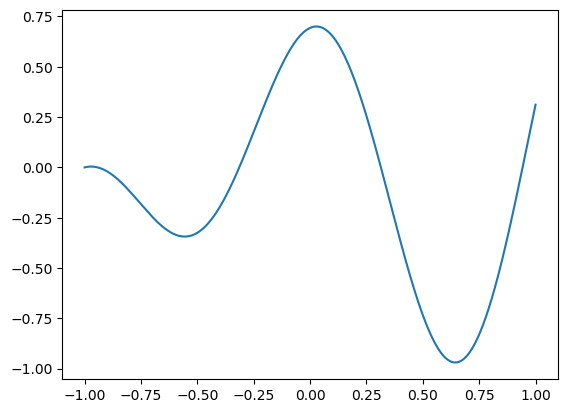
\includegraphics[scale=0.7]{przyklad_f}
	\end{center}
	\caption{Wykres funkcji f}
\end{figure}
\noindent Aby unaocznić zadanie aproksymacji pokazuję wykres wielomianu $W_5$ dla wskazanej funkcji. Czerwone punkty to punkty alternansu. \\
\begin{figure}[H]
	\begin{center}
	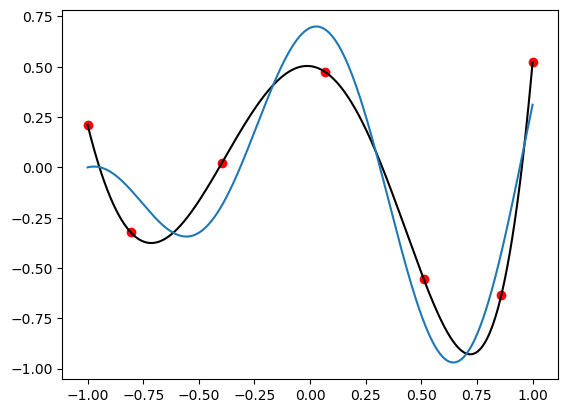
\includegraphics[scale=0.7]{przyklad_W}
	\end{center}
	\caption{Aproksymacja wielomianem optymalnym W}
\end{figure}


\section{Wielomian interpolacyjny $I_n$}
Wielomian $I_n$ jest wielomianem interpolacyjnym stopnia $n$, który interpoluje zadaną funkcję $f$ w punktach $t_{n,k}$ zadanych wzorem
\begin{equation} \label{Zera}
t_{n,k} = \cos \frac{(2k-1)\pi}{2n},
\end{equation}
które są zerami $n$-tego wielomiany Czebyszewa. Wielomian ten bierzemy nie bez powodu, ponieważ spośród wszystkich wielomianów interpolacyjnych chcielibyśmy znaleźć taki, żeby jego norma była najmniejsza, a wiemy z \cite{i1}, że 
\begin{equation}
||f - I_n||_{\infty} \leq \frac{1}{(n+1)!} ||Z||_{\infty} ||f^{(n+1)}||_{\infty}
\end{equation}
gdzie $Z$ jest wielomianem $(n+1)$-tego stopnia. Tak więc norma ta zależy od normy wielomianu $Z$, a najmniejszą normę równą $2^{-n}$ na przedziale $\langle -1, 1 \rangle$ ma wielomian o zerach w zerach wielomanu Czebyszewa  $T_{n+1}$ \cite{i2}. Wielomian interpolujący więc funkcję w zerach Czebyszewa powinien być blisko wielomianu optymalnego. Wielomian ten zadany jest dwoma równoważnymi wzorami\footnote{Wzór na wielomian $I_n$ wziąłem z książki Paszkowskiego i tego się trzymałem pomimo drobnej różnicy względem wzoru podanego na wykładzie.}
\begin{equation} \label{I1}
I_n(x) = \frac{1}{n+1}T_{n+1}(x) \sum_{k=1}^{n+1} (-1)^{k-1}f(t_{n+1,k}) \Big( \sin \frac{(2k-1) \pi}{2(n+1)} \Big) / (x-t_{n+1,k})
\end{equation}
\begin{equation} \label{I2}
I_n(x) = \frac{2}{n+1} \sum_{j=0}^{n} {}^{'} \Big( \sum_{k=1}^{n+1} f(t_{n+1, k}) T_j(t_{n+1, k}) \Big) T_j(x).
\end{equation}
\begin{proof} \cite{i3}
Aby pokazać, że $I_n$ jest wielomianem interpolującym w punktach (\ref{Zera}) rozważmy współczynnik przy $f(t_{n+1,k})$ w (\ref{I1})
\begin{equation}
Q_k(x) = \frac{1}{n+1} T_{n+1}(x) (-1)^{k-1} \sin \frac{(2k-1)\pi}{2(n+1)} / (x - t_{n+1,k})
\end{equation}
Widać, że jest to wielomian, który ma wszystkie zera wielomianu $T_{n+1}$ oprócz $t_{n+1, k}$. Jest to więc wielomian co najwyżej $n$-tego stopnia. Jednocześnie wielomian ten w punktach $t_{n+1, j}$ $j \neq k$ ma wartość $0$.
Możemy też zapisać, że 
\begin{equation}
Q_n(t_{n+1, k}) = \frac{1}{n+1} (-1)^{k+1} \Big( \sin \frac{(2k-1)\pi}{2(n+1)} \Big) T_{n_1}'(t_{n+1,k}),
\end{equation}
a ponieważ
\begin{equation}
T'(t_{n,k}) = (-1)^{k-1} n \Big( \sin \frac{(2k-1)\pi}{2n} \Big)^{-1}
\end{equation}
to $Q_k(t_{n+1, k}) = 1$, więc (\ref{I1}) spełnia warunki interpolacji. Trzeba jeszcze pokazać równoważność dwóch wzorów na wielomian $I_n$. Skorzystamy do tego z równoważności
\begin{equation}
2(x - t_{n+1, k}) \sum_{j=0}^n {}^{'} T_j(t_{n+1, k}) T_j(x) = T_{n+1}(x)T_n(t_{n+1, k})
\end{equation}
gdzie po rozpisaniu $T_n(t_{n+1, k})$ na
\begin{equation}
T_n(t_{n+1, k}) = (-1)^{k-1} \sin \frac{(2k - 1) \pi}{2(n+1)}
\end{equation}
dostajemy, że
\begin{equation}
(-1)^{k-1} \Big( \sin \frac{(2k - 1) \pi}{2(n+1)} \Big) T_{n+1}(x) / (x-t_{n+1, k}) = 2 \sum_{j = 0}^n {}^{'} T_j(t_{n+1, k})T_j(x), 
\end{equation}
więc oba wzory są równoważne.
\end{proof} 
Postanowiłem przetestować możliwości tego wielomianu dla różnych przykładów.
Jednym z nich może być poniższy, w którym aproksymuję funkcję (\ref{przykladowa}) naszym wielomianem: \\ 
\begin{figure}[H]
	\begin{center}
	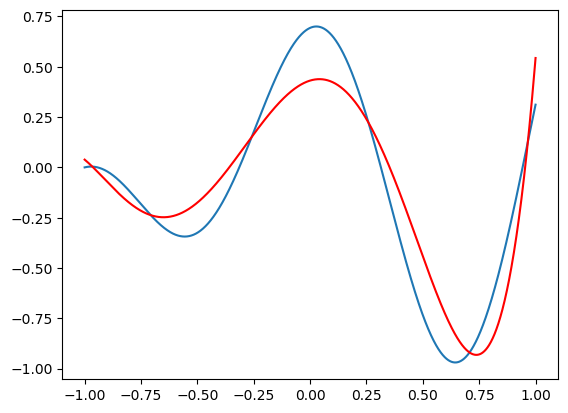
\includegraphics[scale=0.7]{przyklad_I}
	\end{center}
	\caption{Aproksymacja wielomianem I}
\end{figure}
\noindent Wydaje się, że wykres naszego wielomianu zachowuje się tak, jak byśmy chcieli, czyli jest podobny do wykresu wielomianu optymalnego. Wykres błędu naszego wielomianu wygląda tak: \\
\begin{figure}[H]
	\begin{center}
	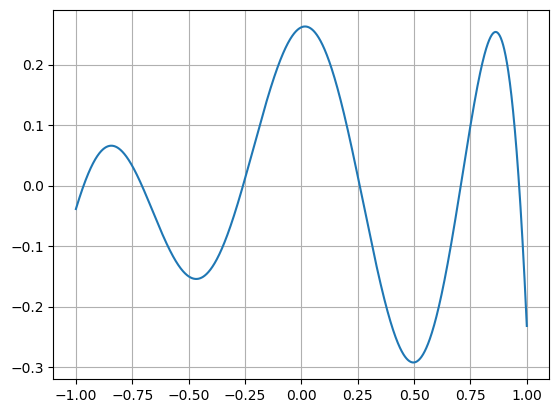
\includegraphics[scale=0.7]{blad_I}
	\end{center}
	\caption{Wykres błędu aproksymacji wielomianem I}
\end{figure}
\noindent Po wykresie widać jednak, że nie można tu pokazać alternansu, więc z twierdzenia Czebyszewa o alternansie nie może to być wielomian optymalny, co dodatkowo widać, gdy porówna się maksymalny błąd. Błąd naszego wielomianu $I_5$ wynosi $0.29226$, podczas gdy błąd wielomiany optymalnego wynosił $0.21101$. Przeprowadziłem jeszcze inne testy dla różnych funkcji, których wyniki przedstawiłem w rozdziale \ref{wyniki}.


\section{Wielomian interpolacyjny $J_n$}
Innym podejściem do aproksymacji może być próba interpolacji funkcji w ekstremach Czebyszewa, czyli w zerach wielomianów Czebyszewa drugiego rodzaju, zadanych wzorem
\begin{equation}
u_{n-1, k} = \cos \frac{k\pi}{n}
\end{equation}
Okazuje się, że dla niektórych funkcji aproksymowanych wielomian $J_n$ interpolujący w tych punktach zachowuje się lepiej niż wielomian $I_n$.  Wielomian $J_n$ wyraża się wzorem
\begin{equation}
J_n(x) = \frac{2}{n} \sum_{j=0}^{n} {}^{''} \Big( \sum_{k=0}^n {}^{''} f(u_{n-1, k})T_j(u_{n-1,k})\Big) T_j(x).
\end{equation}
\begin{proof} \cite{j1}
Przekształćmy wzór na $J_n$ do postaci
\begin{equation}
J_n(x) = \frac{2}{n} \sum_{j=0}^{n} {}^{''} \Big( \sum_{k=0}^n {}^{''} T_j(x) T_j(u_{n-1,k})\Big)f(u_{n-1, k}).
\end{equation}
wiemy, że jeśli zdefiniujemy iloczyn skalarny dla wielomianów wzorem
\begin{equation}
\langle f, g \rangle = \sum_{k=0}^n {}^{''} f(x_k) g(x_k),
\end{equation}
to
\begin{equation}
\langle T_k, T_l \rangle =
\begin{cases}
0 \qquad (k \neq l) \\
n \qquad (k = l = 0 \;\text{lub}\; k = l = n) \\
\frac{n}{2} \qquad (0 < k = l < n),
\end{cases}
\end{equation}
więc biorąc pod uwagę dzielenie pierwszego i ostatniego wyrazu sumy przez 2 w zewnętrznej sumie widzimy, że $f(u_{n-1, k}) = J_n(u_{n-1,k})$.
\end{proof}
Wróćmy znowu do naszej funkcji (\ref{przykladowa}). Wykres aproksymacji prezentuje się następująco: 
\begin{figure}[H]
	\begin{center}
	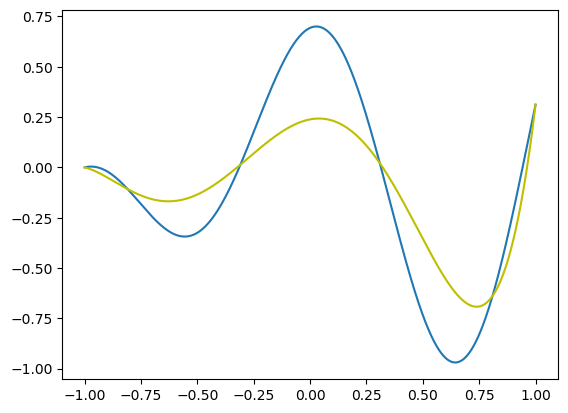
\includegraphics[scale=0.7]{przyklad_J}
	\end{center}
	\caption{Aproksymacja wielomianem J}
\end{figure} 
\noindent natomiast wykres błedu wygląda tak: 
\begin{figure}[H]
	\begin{center}
	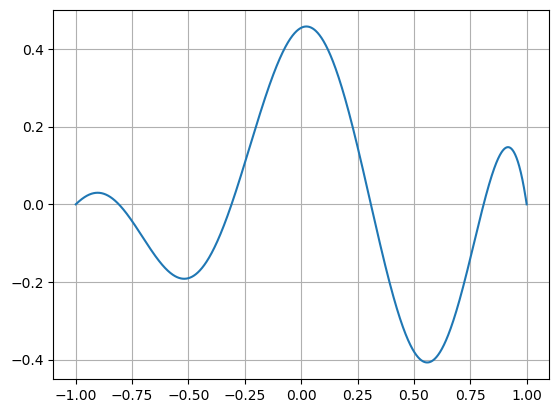
\includegraphics[scale=0.7]{blad_J}
	\end{center}
	\caption{Błąd aproksymacji wielomianem J}
\end{figure}
Wygląda na to, że nasz wielomian $J_5$ aproksymuje znacznie gorzej niż wielomian $I_5$ i widać to już po samym wykresie, a wykres błędu tylko potwierdza nasze podejrzenia. Natomiast po jednym przykładzie nie można jeszcze tak od razu stwierdzić, że $J_n$ jest gorszy. Dlatego zrobiłem więcej testów, a ich wyniki przedstawiłem w rozdziale \ref{wyniki}.


\section{Wielomian $K_n$}
Ostatnim badanym przeze mnie wielomianem był wielomian $K_n$. Wiemy, że aby wielomian $W_n$ był $n$-tym wielomianem optymalnym w sensie aproksymacji jednostajnej, musi posiadać $(n+2)$ punktowy alternans, w którym wartość błędu na zmianę przyjmuje maksymalną wartość błędu. Wielomian $K_n$ jest tak zadany, że gdyby dla wielomianu $W_n$ alternans wypadał by na zbiorze
\begin{equation} \label{zbior}
\{u_{n, 0}, u_{n, 1}, \dots, u_{n, n+1}\}
\end{equation}
to $W_n = K_n$. Wzór na wielomian $K_n$, to
\begin{equation}
K_n(x) = \frac{1}{n+1} \sum_{k=0}^{n+1} {}^{''} (-1)^k f(u_{n,k}) ((x^2-1)U_n(x) / (x-u_{n,k}) - T_{n+1}(x))
\end{equation}
oraz
\begin{equation} \label{K2}
K_n(x) = \frac{2}{n+1} \sum_{j=0}^{n+1} {}^{'} \Big( \sum_{k=0}^{n+1} {}^{''} f(u_{n,k}) T_j(u_{n,k})\Big) T_j(x),
\end{equation}
a $n$-ty bład aproksymacji na zbiorze (\ref{zbior}) wynosi
\begin{equation}
\epsilon = \frac{1}{n+1} \Big| \sum_{k=0}^{n+1} {}^{''} (-1)^k f(u_{n,k}) \Big|.
\end{equation}
\begin{proof} \cite{k1}
Innym wzorem na $J_n$ z poprzedniego rozdziału jest wzór
\begin{equation}
J_{n+1}(x) = \frac{1}{n+1}(x^2-1)U_n(x) \sum_{k=0}^{n+1} {}^{''} 9-1)^kf(u_{n,k})/(x-u_{n,k}).
\end{equation}
Współczynnik stojący przy $x^{n+1}$ w $J_{n+1}$ wynosi
\begin{equation}
\frac{2^n}{n+1} \sum_{k=0}^{n+1} {}^{''} (-1)^kf(u_{n,k}).
\end{equation}
Natomiast poniważ $T_{n+1}(x) = 2^nx^{n+1} + \dots$, więc różnica
\begin{equation}
J_{n+1} - \Big( \frac{1}{n+1} \sum_{k=0}^{n+1} {}^{''} (-1)^kf(u_{n,k}) \Big) T_{n+1}
\end{equation}
jest wielomianem stopnia co najwyżej $n$-tego i jest to przy okazji nasz wielomian $K_n$. Jednocześnie widać, że w punktach $u_{n,k}$ przyjmuje on wartość
\begin{equation}
f(u_{n,k} - \frac{(-1)^j}{n+1} \sum_{k=0}^{n+1} {}^{''} (-1)^kf(u_{n,k})
\end{equation}
czyli posiada $n+2$ punktowy zbiór na którym przyjmuje na zmianę wartość błędu $\epsilon$. Wzór (\ref{K2}) wynika bezpośrednio z określenia $K_n$ jako 
\begin{align*}
K_n &= J_{n+1} - \epsilon T_{n+1} = \\
&= \frac{2}{n+1} \sum_{j=0}^{n+1} {}^{''} \Big( \sum_{k=0}^{n+1} {}^{''} f(u_{n,k})T_j(u_{n,k}) \Big) T_j \;- \\
&- \frac{1}{n+1} \sum_{k=0}^{n+1} {}^{''} f(u_{n,k})T_{n+1}(u_{n,k})T_{n+1} = \\
&= \frac{2}{n+1} \sum_{j=0}^n {}^{'} \Big(\sum_{k=0}^{n+1} {}^{''} f(u_{n,k})T_j(u_{n,k})\Big)T_j.
\end{align*}
\end{proof}
Ponownie przetestujmy aproksymację funkcji (\ref{przykladowa}). Tym razem na wykresach na czerwono zaznaczam punkty (\ref{zbior}), które tworzą alternans naszego wielomianu. 
\begin{figure}[H]
	\begin{center}
	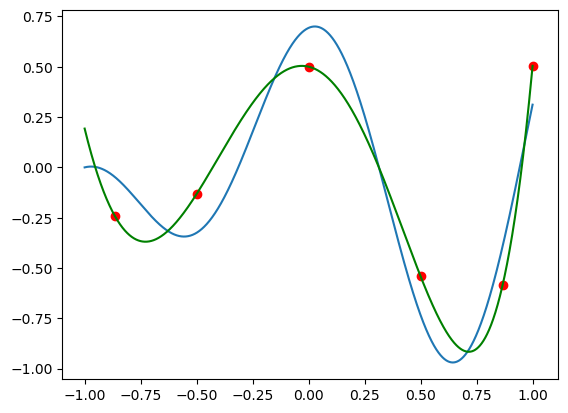
\includegraphics[scale=0.7]{przyklad_K}
	\end{center}
	\caption{Aproksymacja wielomianem K}
\end{figure}
\begin{figure}[H]
	\begin{center}
	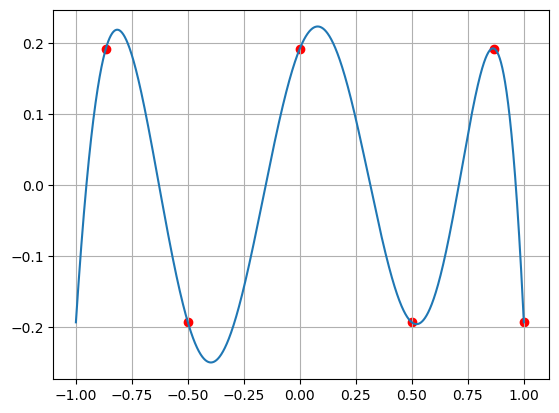
\includegraphics[scale=0.7]{blad_K}
	\end{center}
	\caption{Błąd aproksymacji wielomianem $K_5$.}
\end{figure}
Nasz wielomian $K_5$ wygląda już niemal tak samo, jak wielomian optymalny $W_5$, a wykres błędu pokazuje, że jesteśmy już bardzo blisko tego, aby wielomian ten był wielomianem optymalnym. Widać to również porównując błąd maksymalny, który wynosi $0.24930$ do błedu wielomianu optymalnego $W_5$, a przypomnijmy, że wynosi on $0.21100$. Wydaje się zatem, że jest to bardzo wydajny sposób aproksymacji. Tak jak poprzednie wielomiany przetestowałem ten wielomian dla różnych funkcji, a wyniki przedstawiłem w rozdziale \ref{wyniki}.


\section{Algorytm Clenshowa}
Do liczenia wartości wielomianów postaci
$$ w(x) = \sum_{k=0}^n {}^{'} a_k T_k(x). $$
można użyć algorytmu Clensowa \cite{c1}
\begin{verbatim}
b[n+2] := b[n+1] := 0,
FOR k = n, n-1, ... , 1
    b[k] := a[k] - b[k+2] + 2 * b[k+1] * x
END
RETURN 1/2 * a[0] - b[2] + b[1] * x
\end{verbatim}
Używałem go do liczenia wartości wielomianów $I_n, J_n, K_n$. Aby móc użyć tego kilka razy korzystałem z faktu
\begin{equation}
T_j(u_{n, k}) = T_k(u_{n,j})
\end{equation}
na zbiorze $\langle -1, 1 \rangle$.
\begin{proof}
\begin{align*}
T_j(u_{n,k}) = \cos(n \arccos(u_{n,k})) &= \cos(n \arccos(\cos\Big(\frac{k\pi}{n+1}\Big))) = \\
&= \cos\Big(\frac{nk\pi}{n+1}\Big) = \cos(k \arccos(u_{n,j})) = T_k(u_{n,j})
\end{align*}
\end{proof}


\section{Wyniki testów} \label{wyniki}
Testy, które przeprowadziłem były zautomatyzowane. Wszystkie funkcje były generowane losowo (wielomiany i inne funkcje miały losowe wartości z zadanych przedziałów). Przeprowadziłem testy dla wielomianów, funkcji trygonometrycznych postaci $a \sin x +/* b \cos x$, oraz funkcje mieszane, w których używane były takie funkcje jak $a\log(x+3)$, funkcje trygonometryczne i wielomiany. Zależało mi, aby wszystkie funkcje wygenerowane automatycznie były ciągłe na $\langle -1, 1 \rangle$, dlatego nie ma tu funkcji homograficznych, ani wykładniczych. Aproksymowałem te funkcje wielomianami od stopnia $n = 2, 3, \dots, 100$ w przypadku wielomianów (zatrzymałem testy, w momencie kiedy wartości błędów były bliskie 0) oraz $n = 2,3,\dots, 10$ dla pozostałych funkcji. Na wykresach przedstawiłem moje wyniki:
\begin{enumerate}[•]
\item Dla wielomianów
\begin{figure}[H]
	\begin{center}
	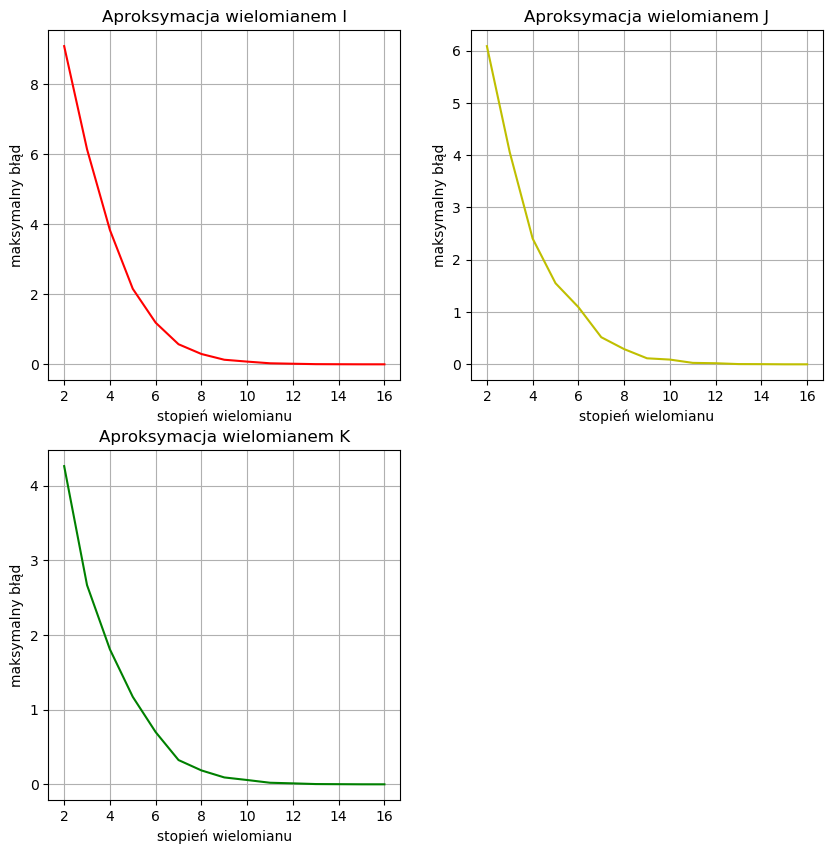
\includegraphics[scale=0.8]{testy_wielomiany}
	\end{center}
\end{figure}
\newpage
\item Dla funkcji trugonometrycznych 
\begin{figure}[H]
	\begin{center}
	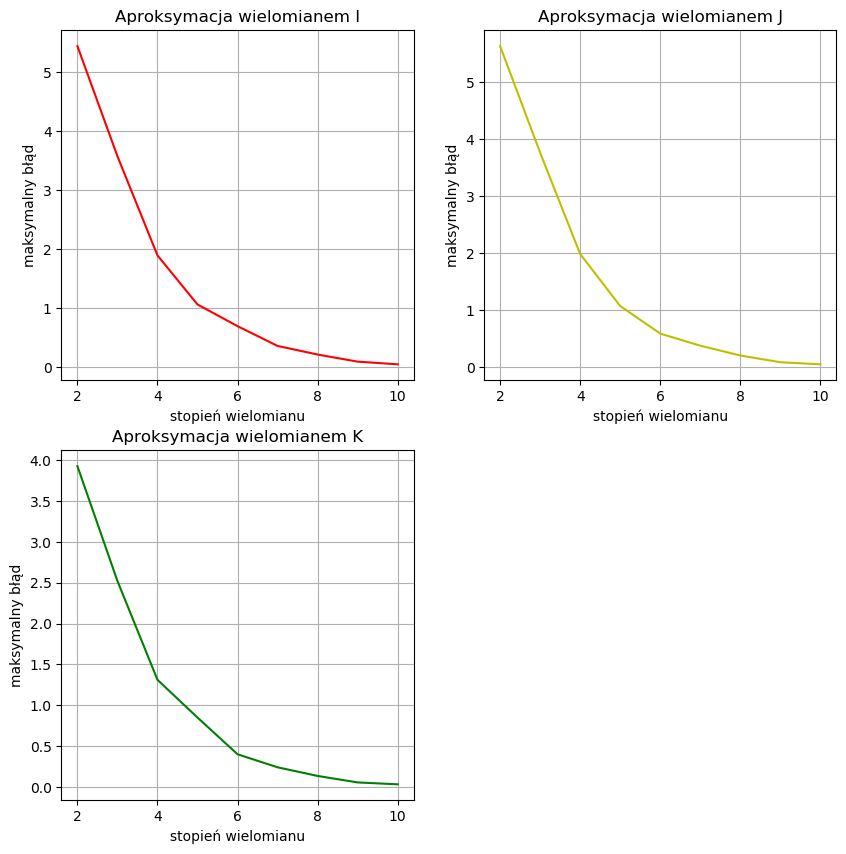
\includegraphics[scale=0.8]{testy_tryg}
	\end{center}
\end{figure}
\newpage
\item Dla funkcji mieszanych 
\begin{figure}[H]
	\begin{center}
	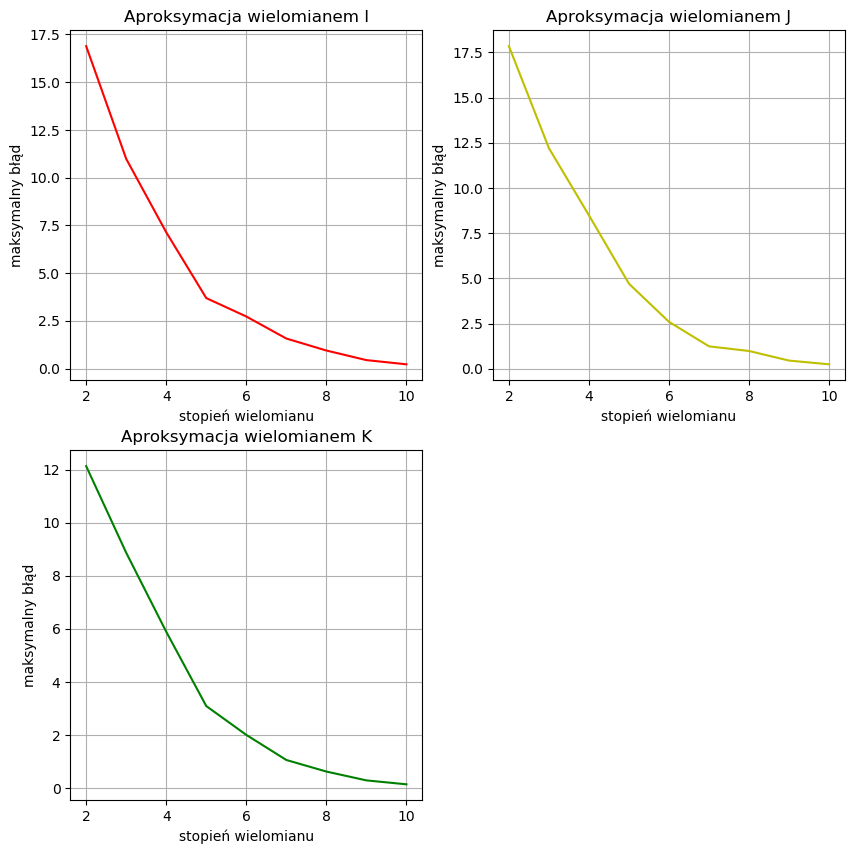
\includegraphics[scale=0.8]{testy_rozne}
	\end{center}
\end{figure}
\end{enumerate}


\section{Podsumowanie i wnioski}
Nietrudno było zauważyć, że wielomian $K_n$ zdecydowanie lepiej się zachowywał niż wielomiany $I_n$ i $J_n$. Wykres błędu tego wielomianu często przypomina taki, który pownien posiadać wielomian optymalny, jego błąd bardzo szybko maleje wraz ze wzrostem wartości $n$. Dzięki algorytmowi Clenshowa policzenie jego wartości okazuje się łatwym zadaniem, co jest kolejnym argumentem przemawiającym na korzyść tego wielomianu.\\
Jeśli zaś chodzi o wielomiany interpolacyjne, ich zachowanie przez cały czas było dość podobne. Widać, że wartości błędu maleją z podobną predkością wraz ze wzrostem wartości $n$, a jeśli chodzi o błędy to na wykresach widać, że są dość zbliżone i chociaż czasami (jak w przypadku wielomianów) wygląda na to, że wielomian $I_n$ jest gorszy, to dla innych funkcji (innych ziaren w losowej generacji) można było zaobserwować, że jest na odwrót. Podobnie z innymi wykresami. Należy więc przyjąć, że wielomiany te dają bardzo zbliżone wartości błędów. Na korzyść wielomianu $J_n$ przemawia jednak jego prostota liczenia dzięki algorytmowi Clenshowa. We wzorze na wielomian $I_n$ mamy sumę postaci
\begin{equation*}
\sum_{k=1}^{n+1} f(t_{n+1, k})T_j(t_{n+1, k}),
\end{equation*}
którego nie można policzyć tym algorytmem, co oznacza, że liczenie wartości $I_n$ jest znacznie trudniejsze. Dlatego, ponieważ zachowują się one tak podobnie, lepiej jest chyba używać wielomianu $J_n$ jeżeli oczywiście nie chcemy  używać wielomianu $K_n$.

\begin{thebibliography}{99}
\bibitem{w1} Na podstawie Stefan Paszkowski „Zastosowania numeryczne wielomianów i szeregów Czebyszewa” wyd. 1975 wstęp do rozdziału 6.
\bibitem{i1} Stefan Paszkowski „Zastosowania numeryczne wielomianów i szeregów Czebyszewa” wyd. 1975 twierdzenie T7.8.
\bibitem{i2} Stefan Paszkowski „Zastosowania numeryczne wielomianów i szeregów Czebyszewa” wyd. 1975 twierdzenie T6.3.
\bibitem{i3} Twierdzenie i dowód Stefan Paszkowski „Zastosowania numeryczne wielomianów i szeregów Czebyszewa” wyd. 1975 T7.9.
\bibitem{j1} Twierdzenie i dowód Stefan Paszkowski „Zastosowania numeryczne wielomianów i szeregów Czebyszewa” wyd. 1975 T7.11.
\bibitem{k1} Twierdzenie i dowód Stefan Paszkowski „Zastosowania numeryczne wielomianów i szeregów Czebyszewa” wyd. 1975 T7.13.
\bibitem{c1} Stefan Paszkowski „Zastosowania numeryczne wielomianów i szeregów Czebyszewa” wyd. 1975 algorytm A14.4, implementacja 19.7.
\end{thebibliography}


\end{document}